% !TeX root = ../thuthesis-example.tex

\chapter{引言}

\section{中微子实验}
中微子是一种电中性、自旋量子数为 1/2 且几乎不与任何物质发射相互作用的一种轻子,只参与弱相互作用与引力相互作用。
作为建立在量子色动力学等学科基础上的粒子物理理论体系,标准模型对粒子历史上许多重要的发现做出了成功的解释或预言。
欧洲核子研究中心(CERN)大型正负电子对撞机(LEP)其中的一个粒子探测器 ALEPH 在 $Z^0$ 共振态附近测量了单光子事例的反应截面\cite{DECAMP1989519},
基于正负电子对撞中唯一稳定的弱相互作用粒子为中微子的前提,得出中微子味道种类 $N_\nu=3.14\pm0.24\enspace(\text{stat.})\pm0.12\enspace(\text{syst.})$.
在持续观测与其他探测器交叉验证后,可以认为自然界只存在三种味道的中微子,分别为对应轻子 $e,\mu,\tau$ 的 $\nu_e,\nu_\mu,\nu_\tau$,及其反粒子。

\begin{figure}
    \centering
    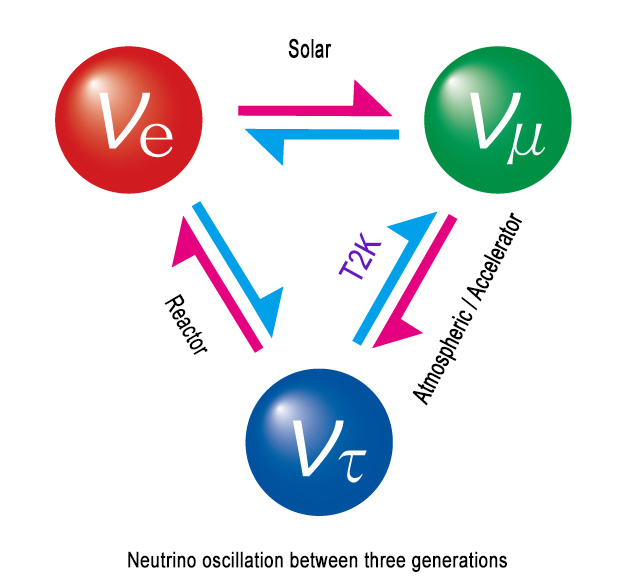
\includegraphics[width=0.65\linewidth]{neutrinos.jpg}
    \caption{中微子振荡}
\end{figure}

在标准模型中,中微子应当没有质量,然而在太阳中微子、大气中微子等中微子实验中均观测到了中微子振荡现象,即中微子在传播过程中存在味的转化,
例如超级神冈在 90\% 置信程度下测量了 $\nu_e\rightarrow\nu_\mu$ 相角与两个质量本征态的质量平方差\cite{fukudaEvidenceOscillationAtmospheric1998},
这意味着中微子必须存在质量。

存在幺正矩阵庞蒂科夫-牧-中川-坂田矩阵(Pontecorvo–Maki–Nakagawa–Sakata matrix 或 PMNS matrix)描述中微子味与质量本征态的关系\cite{Cahn2009Aug}:
\begin{equation}
    \begin{bmatrix}
        v_1&v_2&v_3
    \end{bmatrix}
    =
    \begin{bmatrix}
        v_e&v_\mu&v_\tau
    \end{bmatrix}U.
\end{equation}
\begin{equation}\label{eq:PMNS}
    U=
    \begin{bmatrix}
    c_{12}c_{13}&s_{12}c_{13}&s_{13}e^{-i\delta}\\-s_{12}c_{23}-c_{12}s_{23}s_{13}e^{i\delta}&c_{12}c_{23}-s_{12}s_{23}s_{13}e^{i\delta}&s_{23}c_{13}\\s_{12}s_{23}-c_{12}c_{23}s_{13}e^{i\delta}&-c_{12}s_{23}-s_{12}c_{23}s_{13}e^{i\delta}&c_{23}c_{13}
    \end{bmatrix}
    \times 
    \begin{bmatrix}
    e^{i\alpha_1/2}&0&0\\0&e^{i\alpha_2/2}&0\\0&0&1
    \end{bmatrix}.
\end{equation}

其中引入混合角 $\theta_{ij},\enspace i<j$ 与 $s_{ij}=\sin{\theta_{ij}},\enspace c_{ij}=\cos{\theta_{ij}}$,$\delta$ 为 CP 破坏相角。
~\eqref{eq:PMNS} 除了用来描述尚且未知是否成立的马约拉纳性的 $\alpha_1,\alpha_2$ 部分与卡比博-小林-益川矩阵(Cabibbo–Kobayashi–Maskawa matrix 或 CKM matrix)形式一致,
剩余部分可以写成:
\begin{equation}
    U_{res}=
    \begin{bmatrix}
    1&0&0\\0&c_{23}&s_{23}\\0&-s_{23}&c_{23}
    \end{bmatrix}
    \begin{bmatrix}
    c_{13}&0&s_{13}e^{-i\delta}\\0&1&0\\-s_{13}e^{i\delta}&0&c_{13}
    \end{bmatrix}
    \begin{bmatrix}
    c_{12}&s_{12}&0\\-s_{12}&c_{12}&0\\0&0&1
    \end{bmatrix}.
\end{equation}

$\theta_{12},\theta_{23}$ 都较大而 $\theta_{13}$ 较小,然而正是 $\theta_{13}$ 的存在,中微子震荡中的 CP 破坏才能够显现。
太阳中微子与大气中微子分别能够测量质量平方差:
\begin{align}
    \Delta m_{\text{sol}}^2&=m_2^2-m_1^2\label{eq:sol}\\
    \Delta m_{\text{atm}}^2&=\left|m_3^2-m_1^2\right|\approx\left|m_3^2-m_2^2\right|\label{eq:atm}
\end{align}

目前 $\sin{2\theta_{13}}$ 与 $\delta$ 还需要精细测量,且只有~\eqref{eq:sol} 确定了两个质量相近的质量本征态(2 与 1)的质量顺序,
~\eqref{eq:atm} 并不能确定 $m_3$ 质量的排序位置,还存在正质量顺序 $m_3>m_2>m_1$ 与倒序 $m_2>m_1>m_3$ 两种可能。
不同的质量顺序与质量平方差参数对能谱的形状有直接的影响,为了精细测量参数并确定中微子质量顺序,需要积累足够多的反中微子事例,使用能谱拟合得到置信度到达 $3\sim5\sigma$ 的物理结果。

\begin{figure}
    \centering
    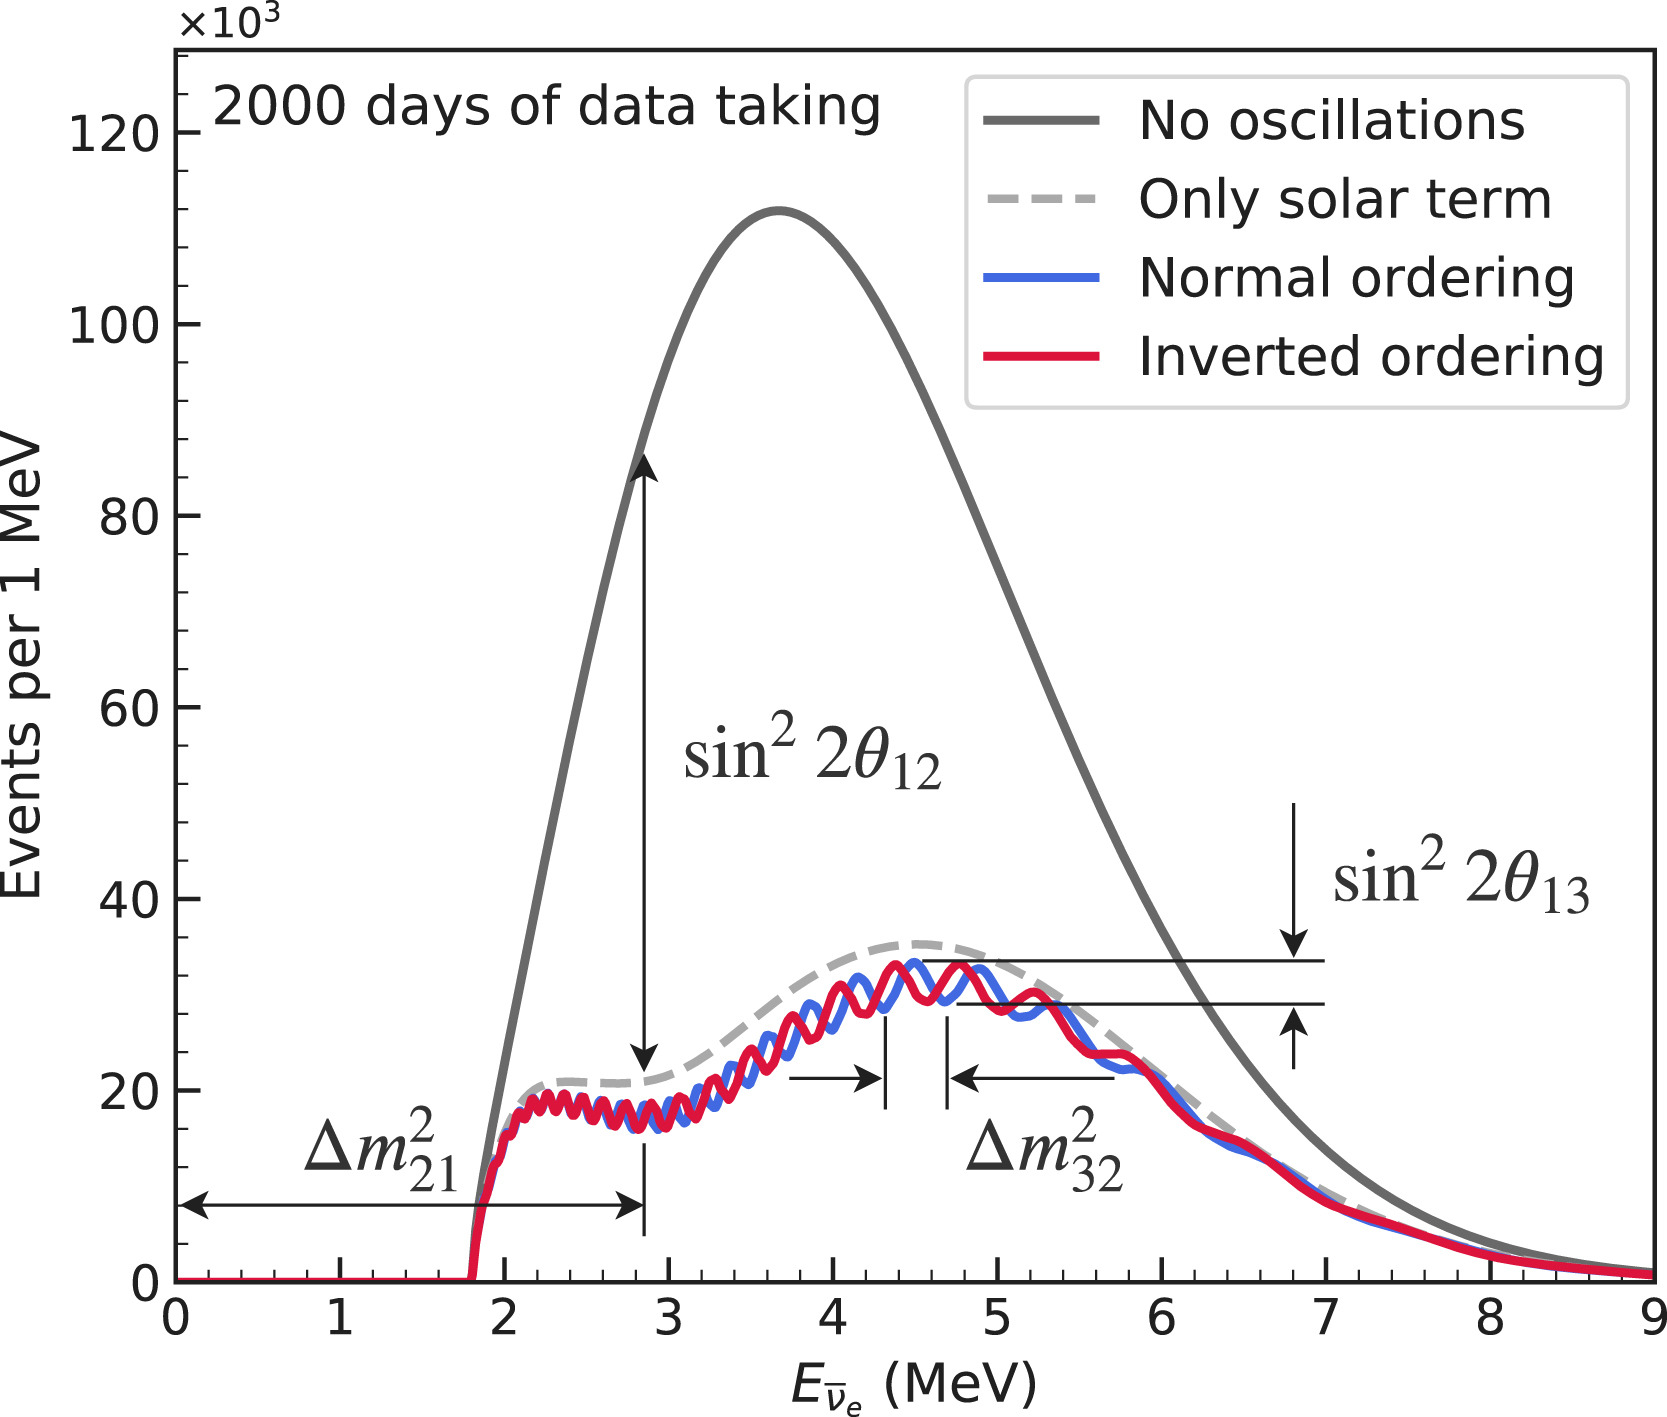
\includegraphics[width=0.65\linewidth]{energy_spectrum.jpg}
    \caption{混合角、质量参数与质量顺序对反中微子能谱的影响\cite{JUNOPhysicsDetector2022}}
\end{figure}

\section{江门中微子实验与 OSIRIS 探测器}\label{sec:osiris}
江门地下中微子观测站(Jiangmen Underground Neutrino Observatory,以下简称 JUNO)\cite{JUNOPhysicsDetector2022}
是位于地表 700 米以下的装载两万吨液体闪烁体的球形探测器,预期达到 $\sigma_E/E=3.02\%/\sqrt{E(\text{MeV})}$ 的能量分辨率,主要物理目标包括:
\begin{itemize}
    \item 利用台山与阳江核电站的反应堆反中微子来确定中微子质量顺序;
    \item 探测地源与地外源的中微子与反中微子事例,例如太阳中微子、大气中微子、地球中微子、超新星中微子等;
    \item 寻找质子衰变 $p\rightarrow K^{+}+\overline{\nu}$、暗物质湮灭致中微子发射等新物理。
\end{itemize}

JUNO 主要探测的物理反应包括:
\begin{align}
    &\overline{\nu}_e+p\rightarrow e^++n \label{eq:ibd}\\
    &\nu+e\rightarrow\nu+e \label{eq:ees}\\
    &\nu+p\rightarrow\nu+p \label{eq:pes}
\end{align}

~\eqref{eq:ibd} 是逆 $\beta$ 衰变反应(inverse beta decay,以下简称 IBD)最主要的探测事例,~\eqref{eq:ees} 与 ~\eqref{eq:pes} 分别为中微子和电子与质子的弹性散射
(elastic neutrino–electron/proton scattering 或 eES 与 pES)。

JUNO 中心装载两万吨液体闪烁体的球体称为中央探测器,使用 5000 支打拿级光电倍增管(dynode photomultiplier tube,以下简称 dynode PMT)
与 12612 支微通道型光电倍增管(microchannel plate photomultiplier tube,以下简称 MCP-PMT)捕获中微子相互作用伴随的微弱闪烁光,
周围使用超纯水包裹并设置水切伦科夫探测器,顶端使用塑料闪烁体阵列。

\begin{figure}
    \centering
    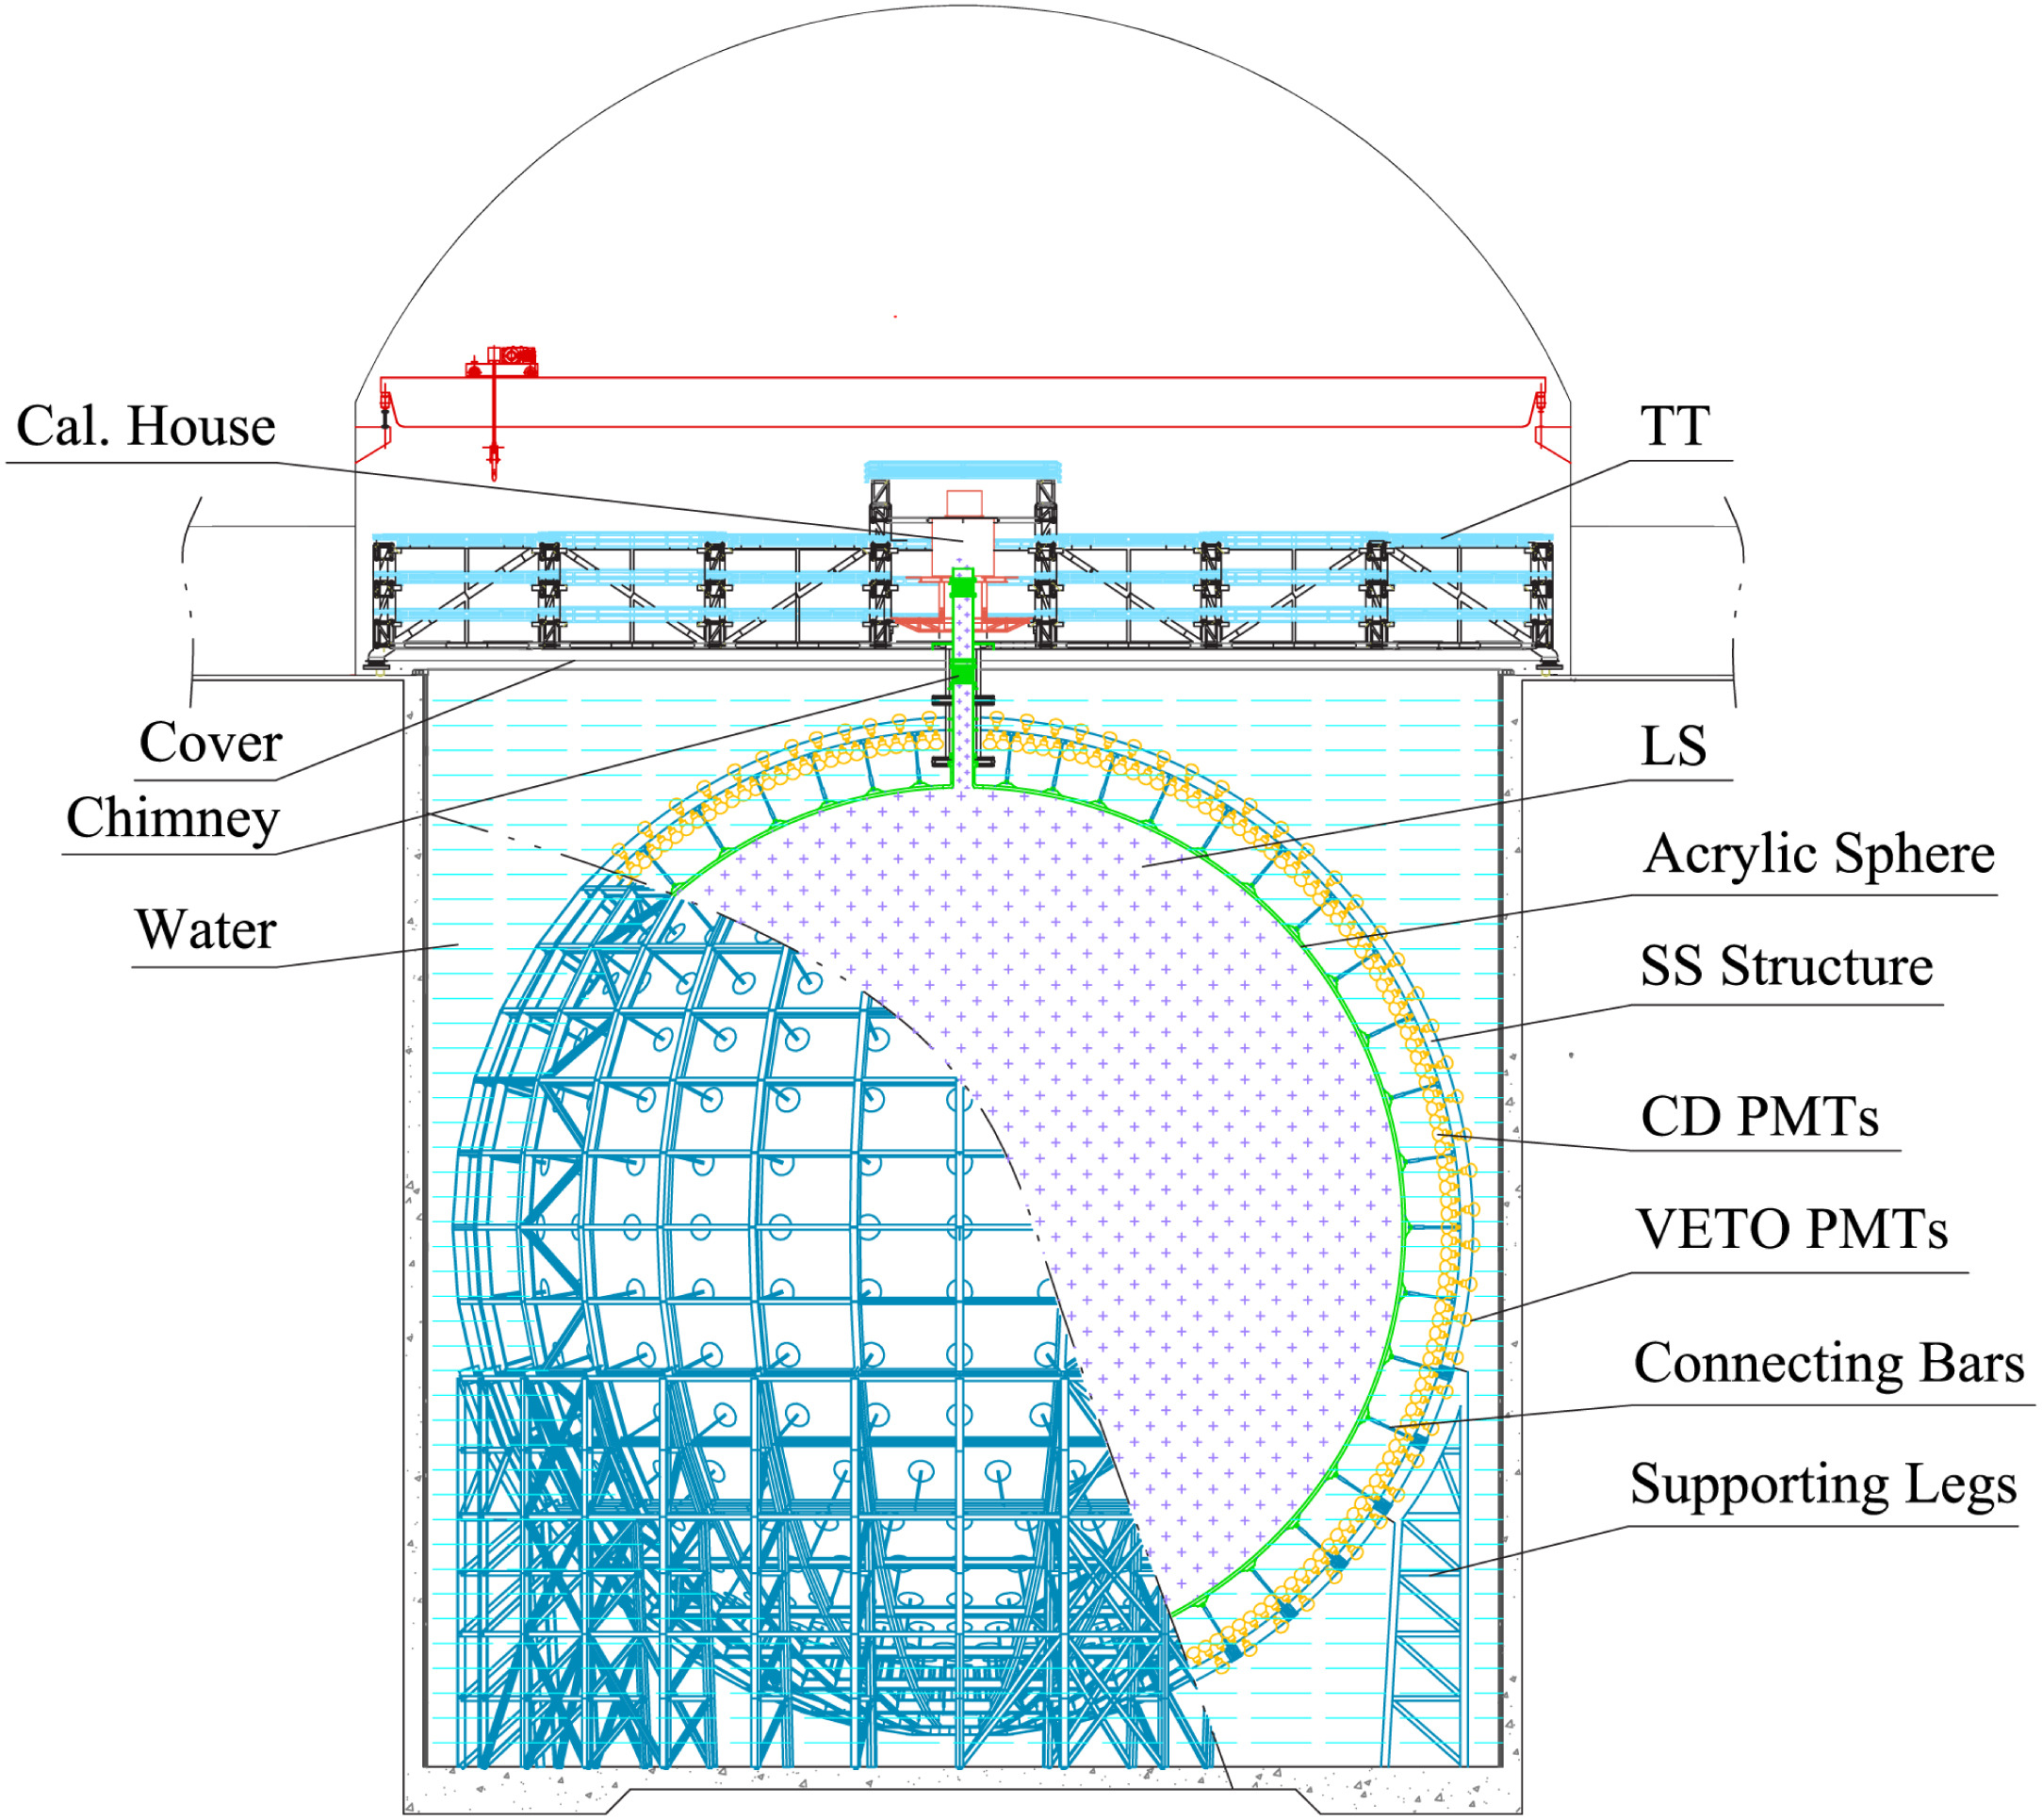
\includegraphics[width=0.85\linewidth]{juno.jpg}
    \caption{JUNO 探测器侧视示意图\cite{JUNOPhysicsDetector2022}}
\end{figure}

液体闪烁体中主要检测介质为线性烷基苯(Linear alkylbenzene 或 LAB),并掺杂
2,5-二苯基噁唑(以下简称 PPO)与 1,4-双(2-甲基苯乙烯基)苯(以下简称 bis-MSB)。
液体闪烁体的放射性纯度与透明度直接影响噪声水平,决定了探测灵敏度的极限,
例如对于反应堆中微子的放射性纯度要求为 $1\times10^{-15}$ g/g,对太阳中微子则为 $1\times10^{-16\sim17}$ g/g。
为了检查液体闪烁体是否达标,在罐装入中心探测器前,需要经过加压氧化铝纯化塔与超纯水萃取塔,掺杂 PPO 与 bis-MSB 后通过水萃取与反萃取系统,
并以 220 nm 与 50 nm 两级过滤器过滤灰尘以及 $^{238}\text{U}$ 与 $^{232}\text{Th}$ 的放射性本底,
最终输入在线闪烁体内部放射性调查系统(Online Scintillator Internal Radioactivity Investigation System,以下简称 OSIRIS)
探测器\cite{junocollaborationDesignSensitivityJUNO2021}进行采数考察。

\begin{figure}
    \centering
    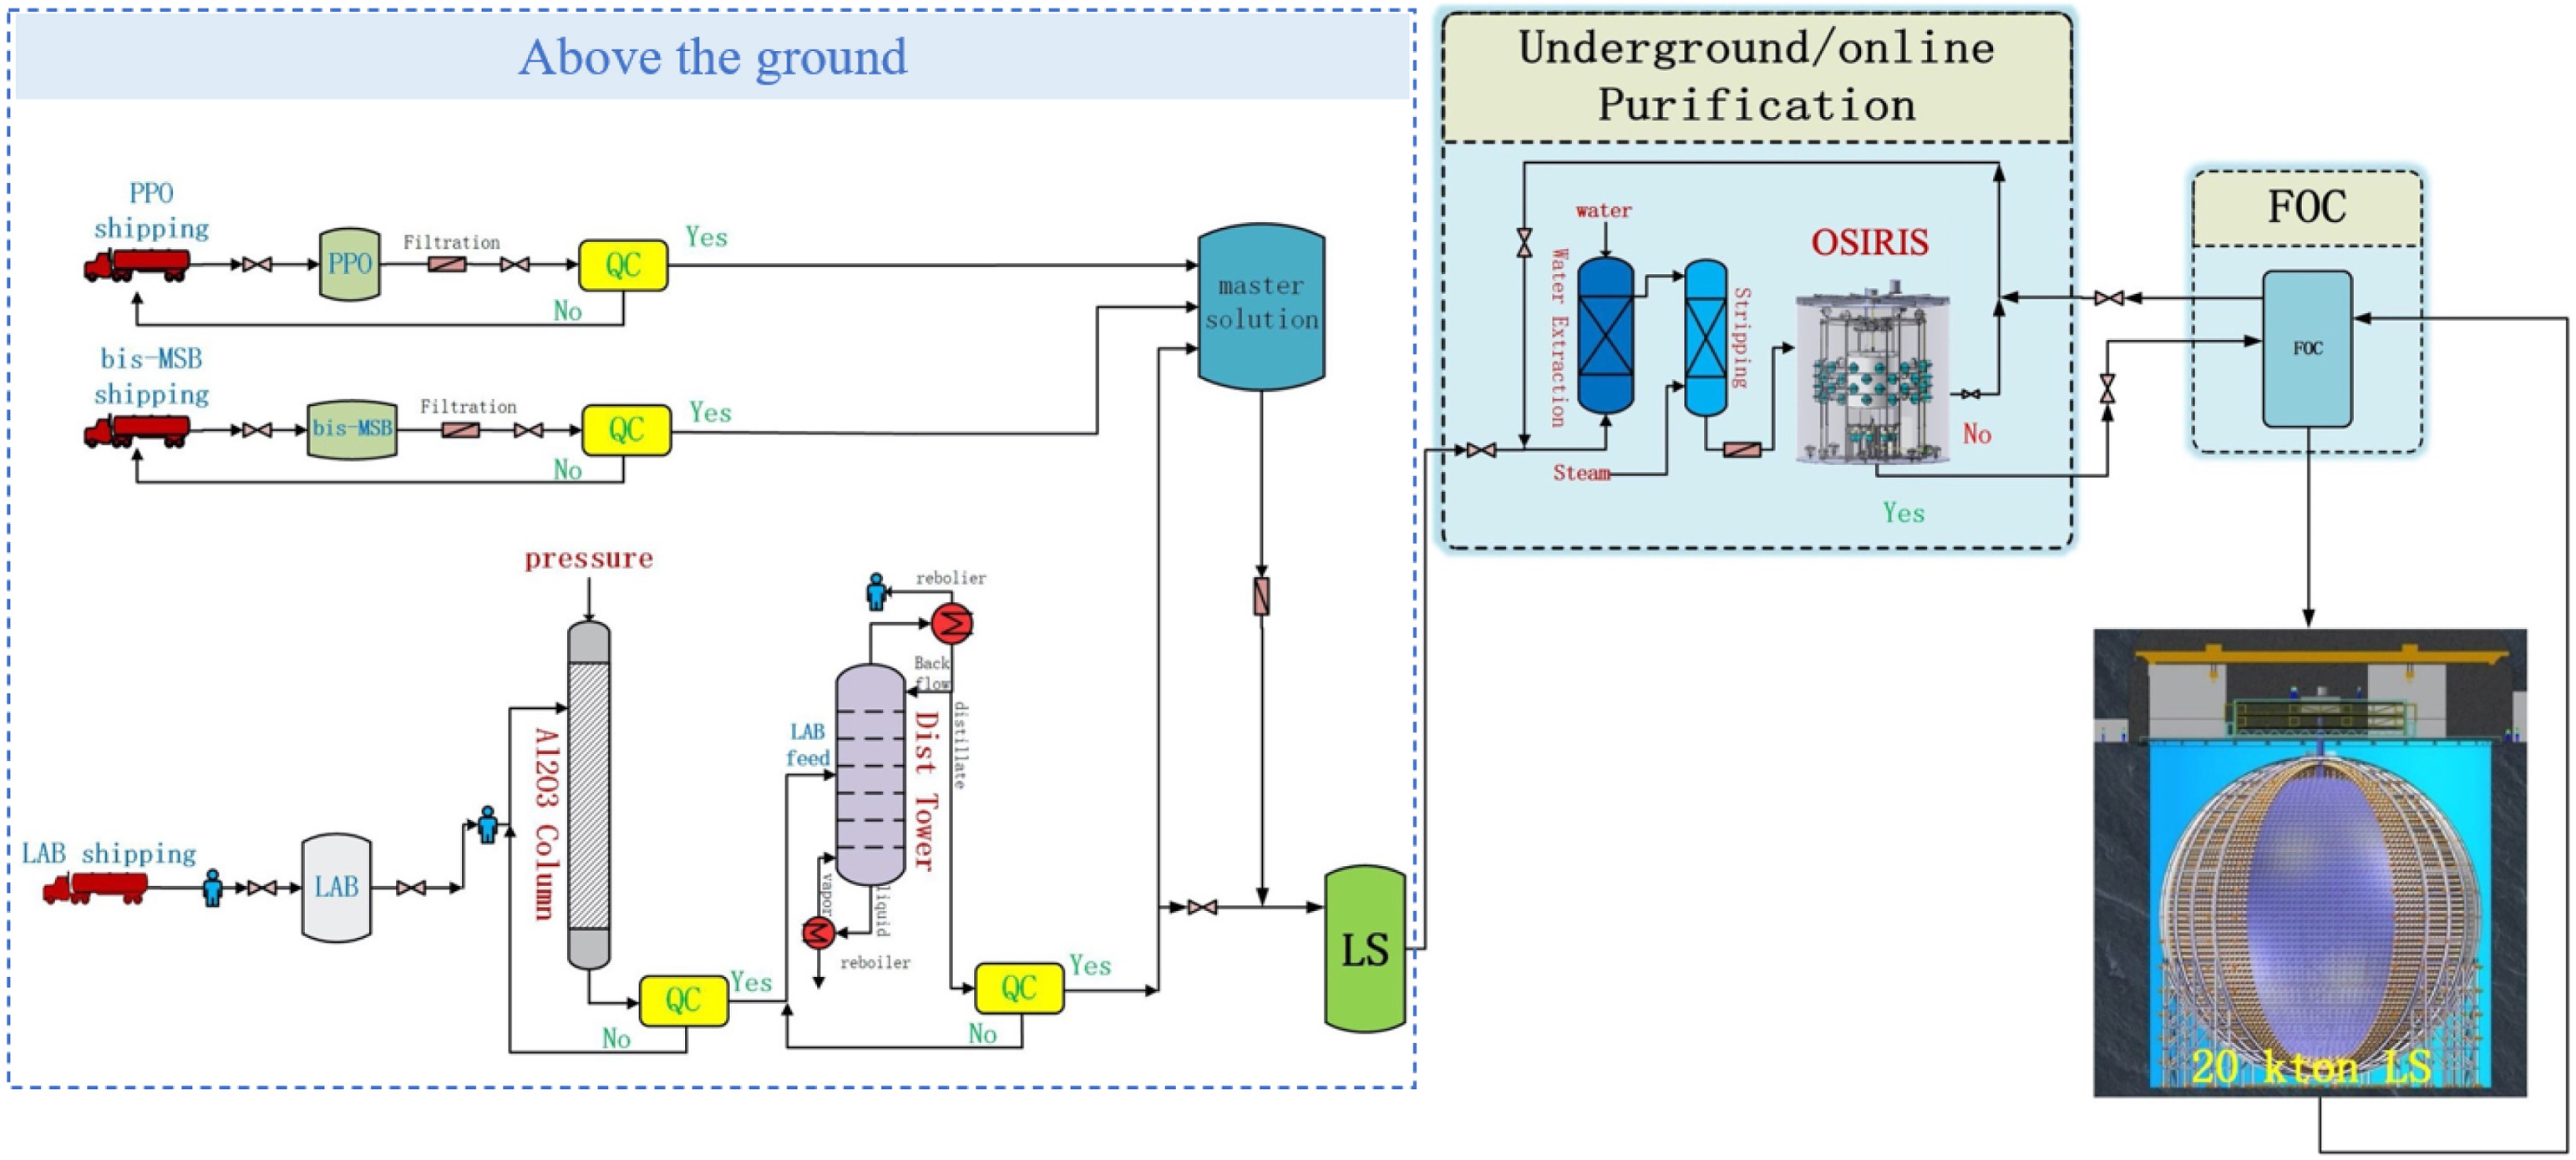
\includegraphics[width=\linewidth]{LS.jpg}
    \caption{液体闪烁体处理系统的流程图}
\end{figure}

OSIRIS 在液体闪烁体循环提纯系统期间,对单批次液体闪烁体展开连续观察,通过研究 U/Th 衰变链中 $^{214}\text{Bi}-^{214}\text{Po}$ 与 
$^{212}\text{Bi}-^{212}\text{Po}$ 的快符合衰变进行纯度分析,直至液体闪烁体纯度达到探测 IBD 反应与太阳中微子的要求。
在 JUNO 中心探测器罐装液体闪烁体期间,OSIRIS 将使用从容纳液体闪烁体的亚克力容器顶部添加新液体闪烁体、从底部引出监测完毕的液体闪烁体的方式,
对其纯度进行连续地分析,灵敏度将达 IBD 反应探测要求。

OSIRIS 为直径与高度均为 9.4 m 的圆柱形探测器,中心使用直径与高度均为 3 m 的亚克力容器灌装液体闪烁体,外围框架使用不锈钢
并使用水填充。在亚克力容器周围,安装有 64 个 20 寸 MCP-PMT,在顶部与底部另有 12 个 20 寸 MCP-PMT 用以排除 $\mu$ 子。
同时,它也具有皮秒脉冲激光系统、放射源与 LED 作为光源的刻度系统,其激光系统的激光脉冲展宽约 80 ps,光纤长度几乎一致,
故光运行时间差异相较于 MCP-PMT 自身的渡越时间展宽(transition time spread, 以下简称 TTS)可以忽略。

\begin{figure}
    \centering
    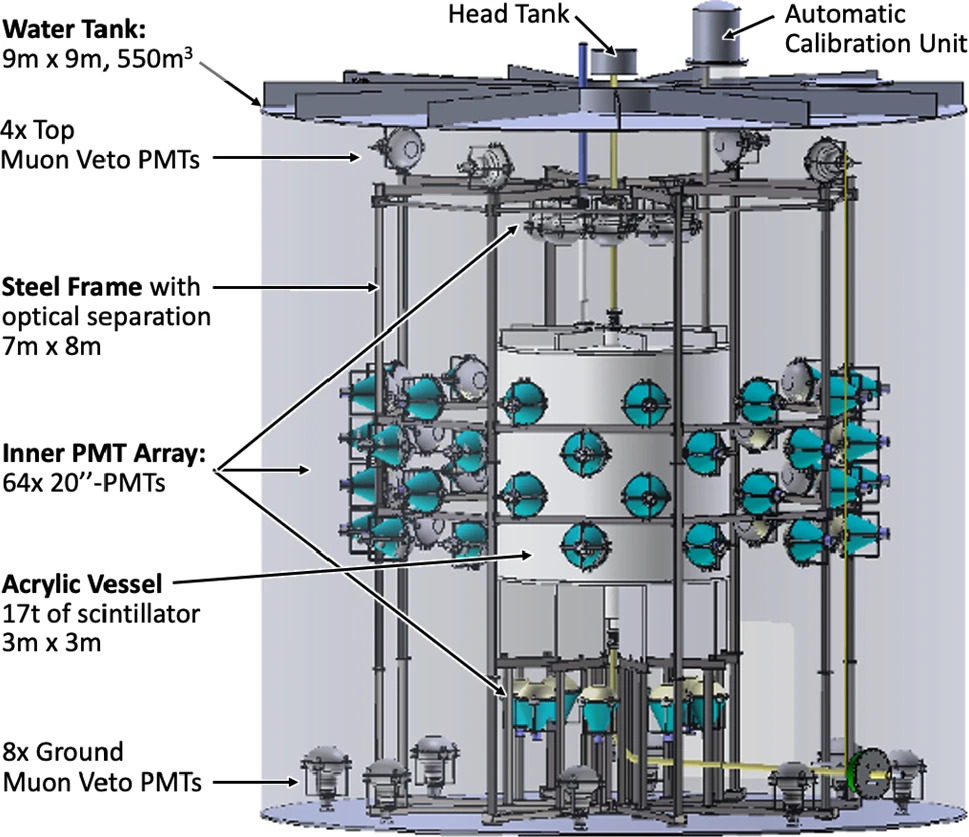
\includegraphics[width=0.7\linewidth]{osiris.jpg}
    \caption{OSIRIS 探测器示意图}
\end{figure}

OSIRIS 的 24 个激光扩散器遍布在不锈钢钢架上,其中 8 个向内安装在亚克力容器赤道平面上,两侧各 4 个安装在亚克力容器的顶部与底部用来照亮对侧的 PMT,
另有 8 个安装在探测器外部框架上。

OSIRIS 探测器已于 2024 年 3 月完成液体闪烁体灌装,完成了 4 次亚克力容器内部液体闪烁体循环,至今积累了近 3 个月的实际数据,
其中包括两轮共计 5 天的激光刻度数据。该工作环境与 JUNO 探测器未来的 PMT 工作环境完全一致,因此该刻度数据对 PMT 的刻度具有重要意义。

\section{新型光电倍增管的特性}
光电倍增管是大型中微子实验的核心器件,它主要用来捕获光信号,来对中微子在液体闪烁体或者水中发生相互作用后释放的光子进行探测。
PMT 相较于半导体探测器等其他探测器件,具有灵敏度高的特点:由于产生载流子需要的能量并不高,
且 PMT 的多级放大能够有效倍增载流子的数量,即使光子数量非常少,
也能够有效地产生大量电子,在 PMT 阳极上接收到显著的电压信号。

为了解决依赖国外公司 PMT 进口的高额成本问题,
中国科学院高能物理研究所、北方夜视技术股份有限公司等单位合作
设计、研究、改进与生产了新型 MCP-PMT,在其量子效率(quantum efficiency,以下简称 QE)系数与收集效率
(collection efficiency,以下简称 CE)系数等方面均做出了改进\cite{wangNewDesignLarge2012}并有效降低了成本。

\begin{figure}
    \centering
    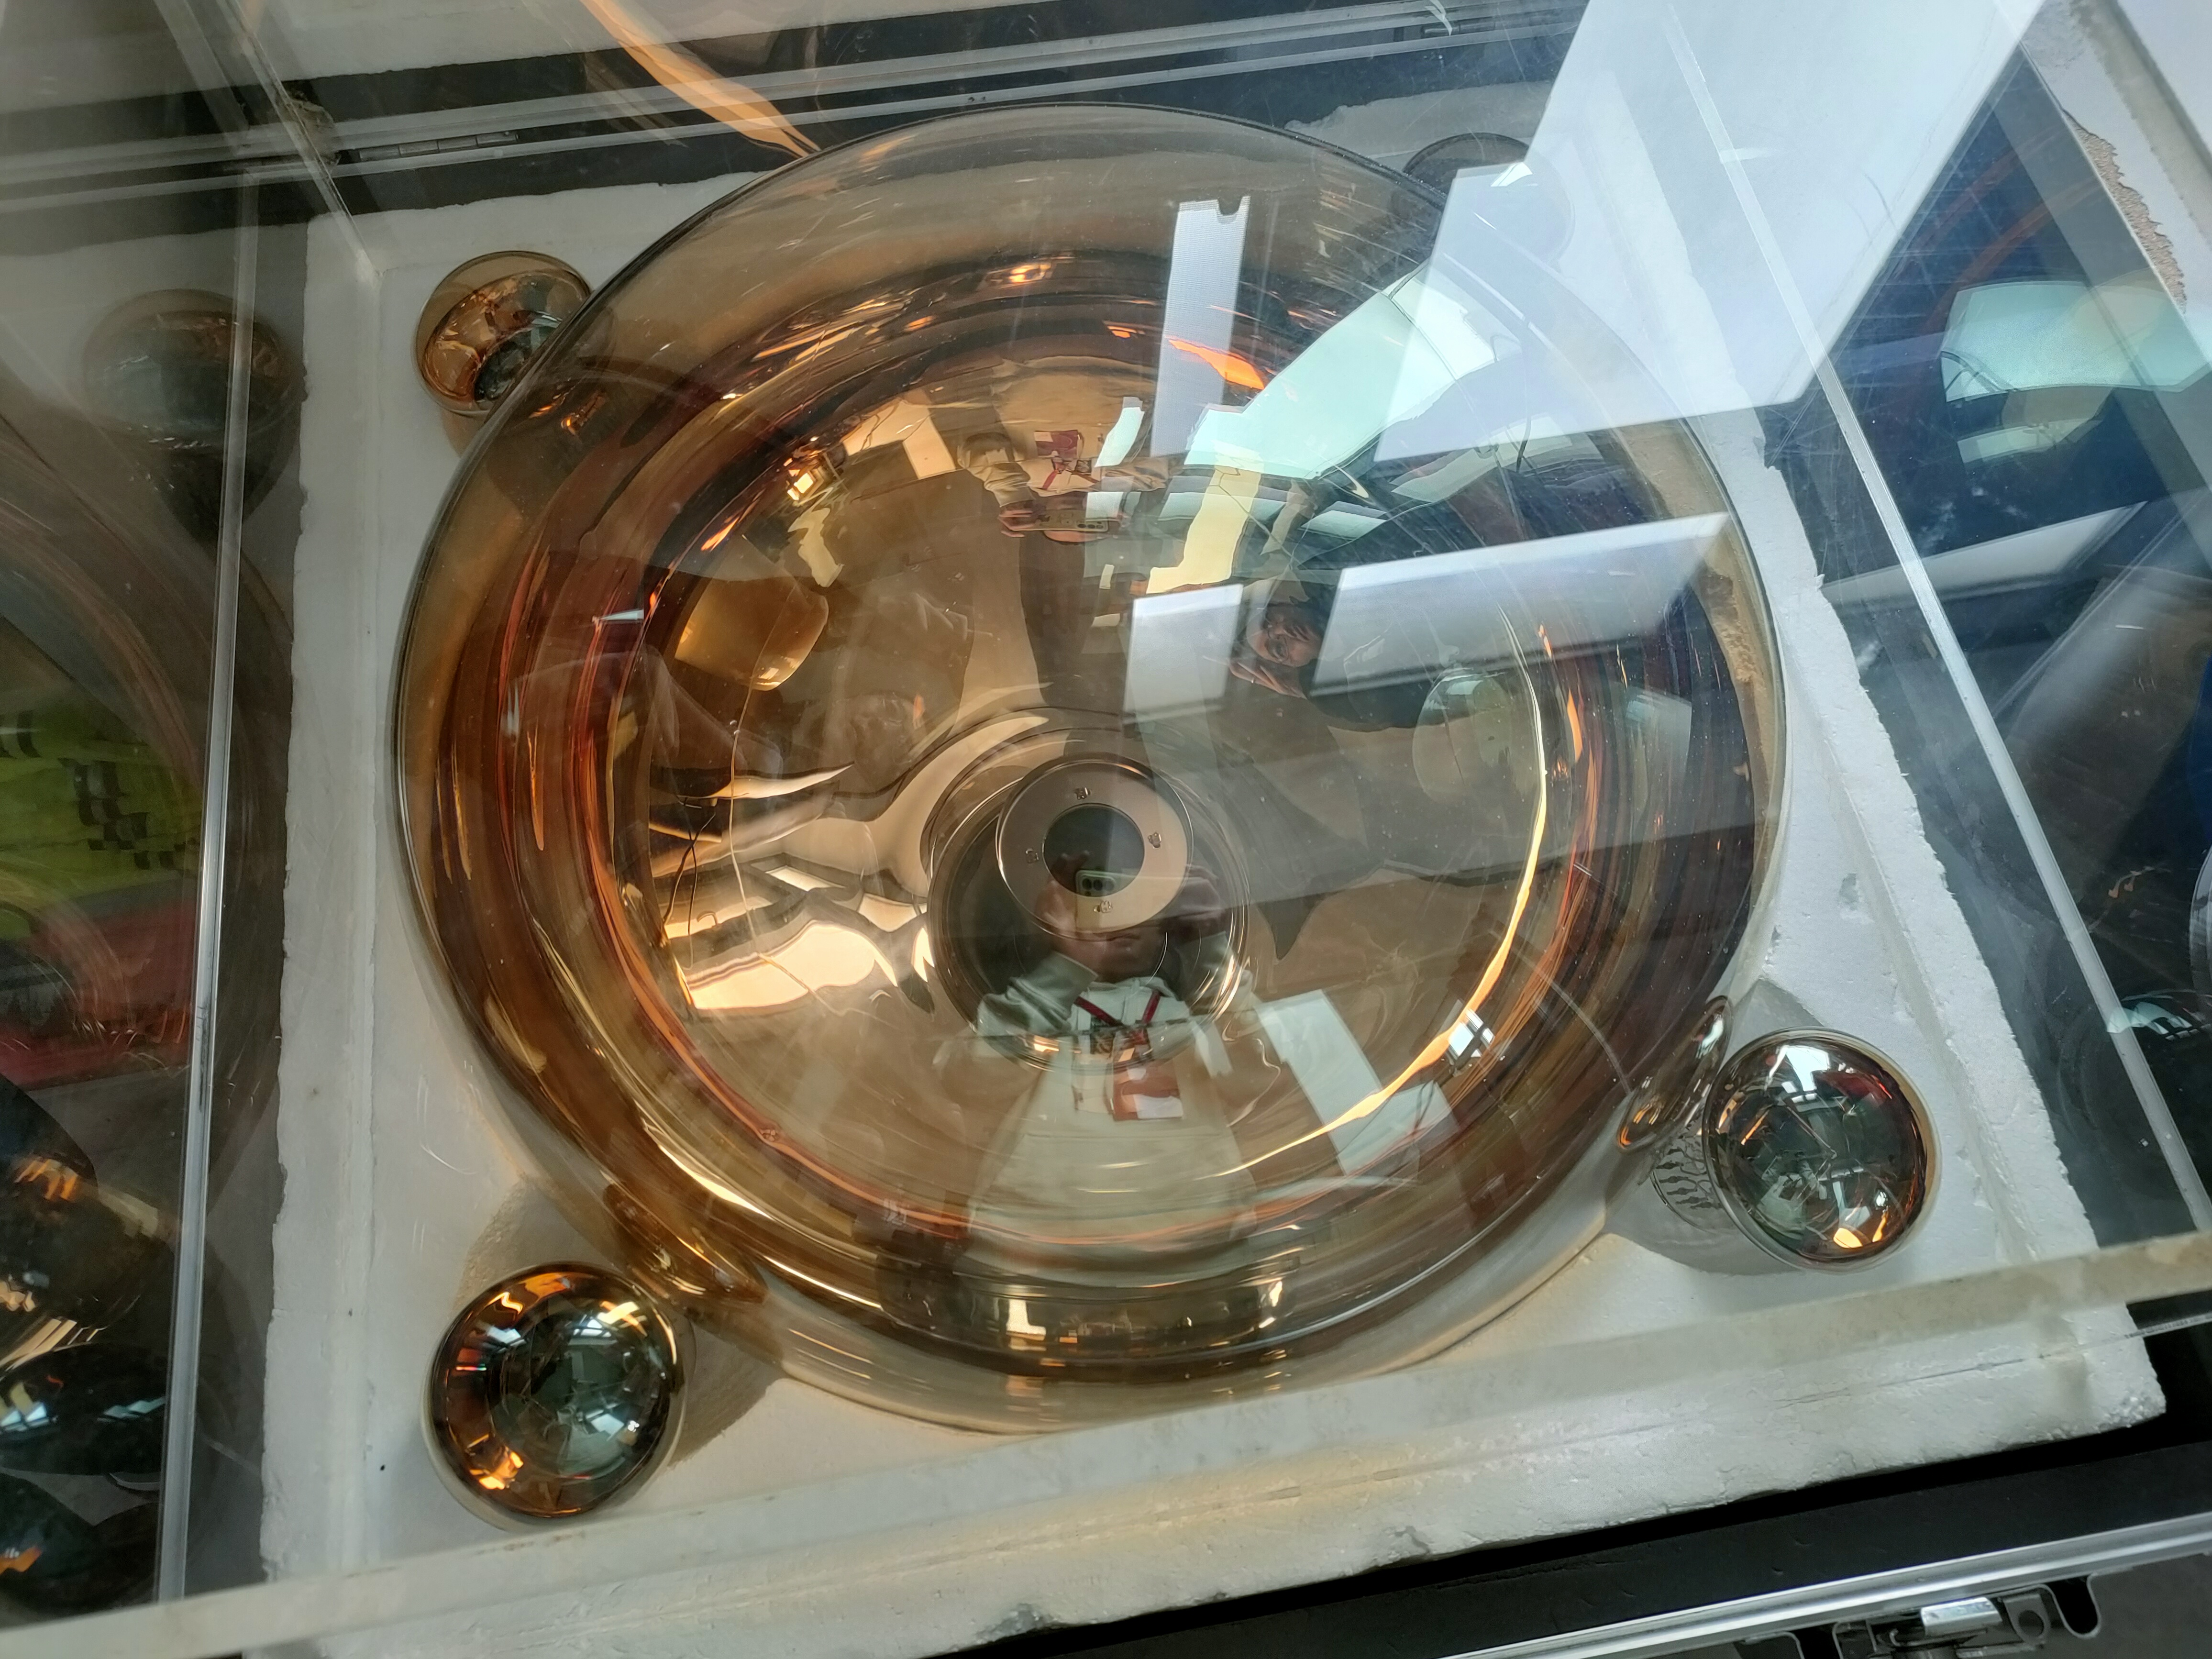
\includegraphics[width=0.7\linewidth]{mcp_pmt.jpg}
    \caption{20 寸 MCP-PMT 与环绕的 4 个 3 寸 MCP-PMT}
\end{figure}

该 MCP-PMT 的突出特点包括:
\begin{enumerate}
    \item 相较于常见的 dynode PMT,使用具有微小倾角的斜长微通道板(microchannel plate,以下简称 MCP)取代了分离式的多级打拿级,
    因此可以发生倍增物理过程的接触点变得连续,PMT 外接高压引线结构得到简化,电子的收集效率也较高;
    \item 相对于其他种类的 MCP-PMT,该 PMT 的特点为在 MCP 表面引入了主要成分为复合 $\text{Al}_2\text{O}_3-\text{MgO}$ 的
    原子沉积涂层(atomic layer deposition,以下简称 ALD),该 ALD 涂层具有高二次电子倍增系数的特点\cite{caoSecondaryElectronEmission2021},
    即电子在该表面具有较高的激发二次电子的概率与二次电子数目的期望;
    \item 单位数目的电子在入射该 MCP-PMT 后,能够产生较一般其他类型 PMT 更多的倍增电子并在阳极被收集(比值定义为 CE),
    因此理论意义上具有更优秀的峰谷比与分辨率;
    \item 由于二次倍增电子的存在,收集到大电荷信号的概率较其他 PMT 高,表现在电荷谱具有“长尾”结构。
\end{enumerate}

\begin{figure}
    \centering
    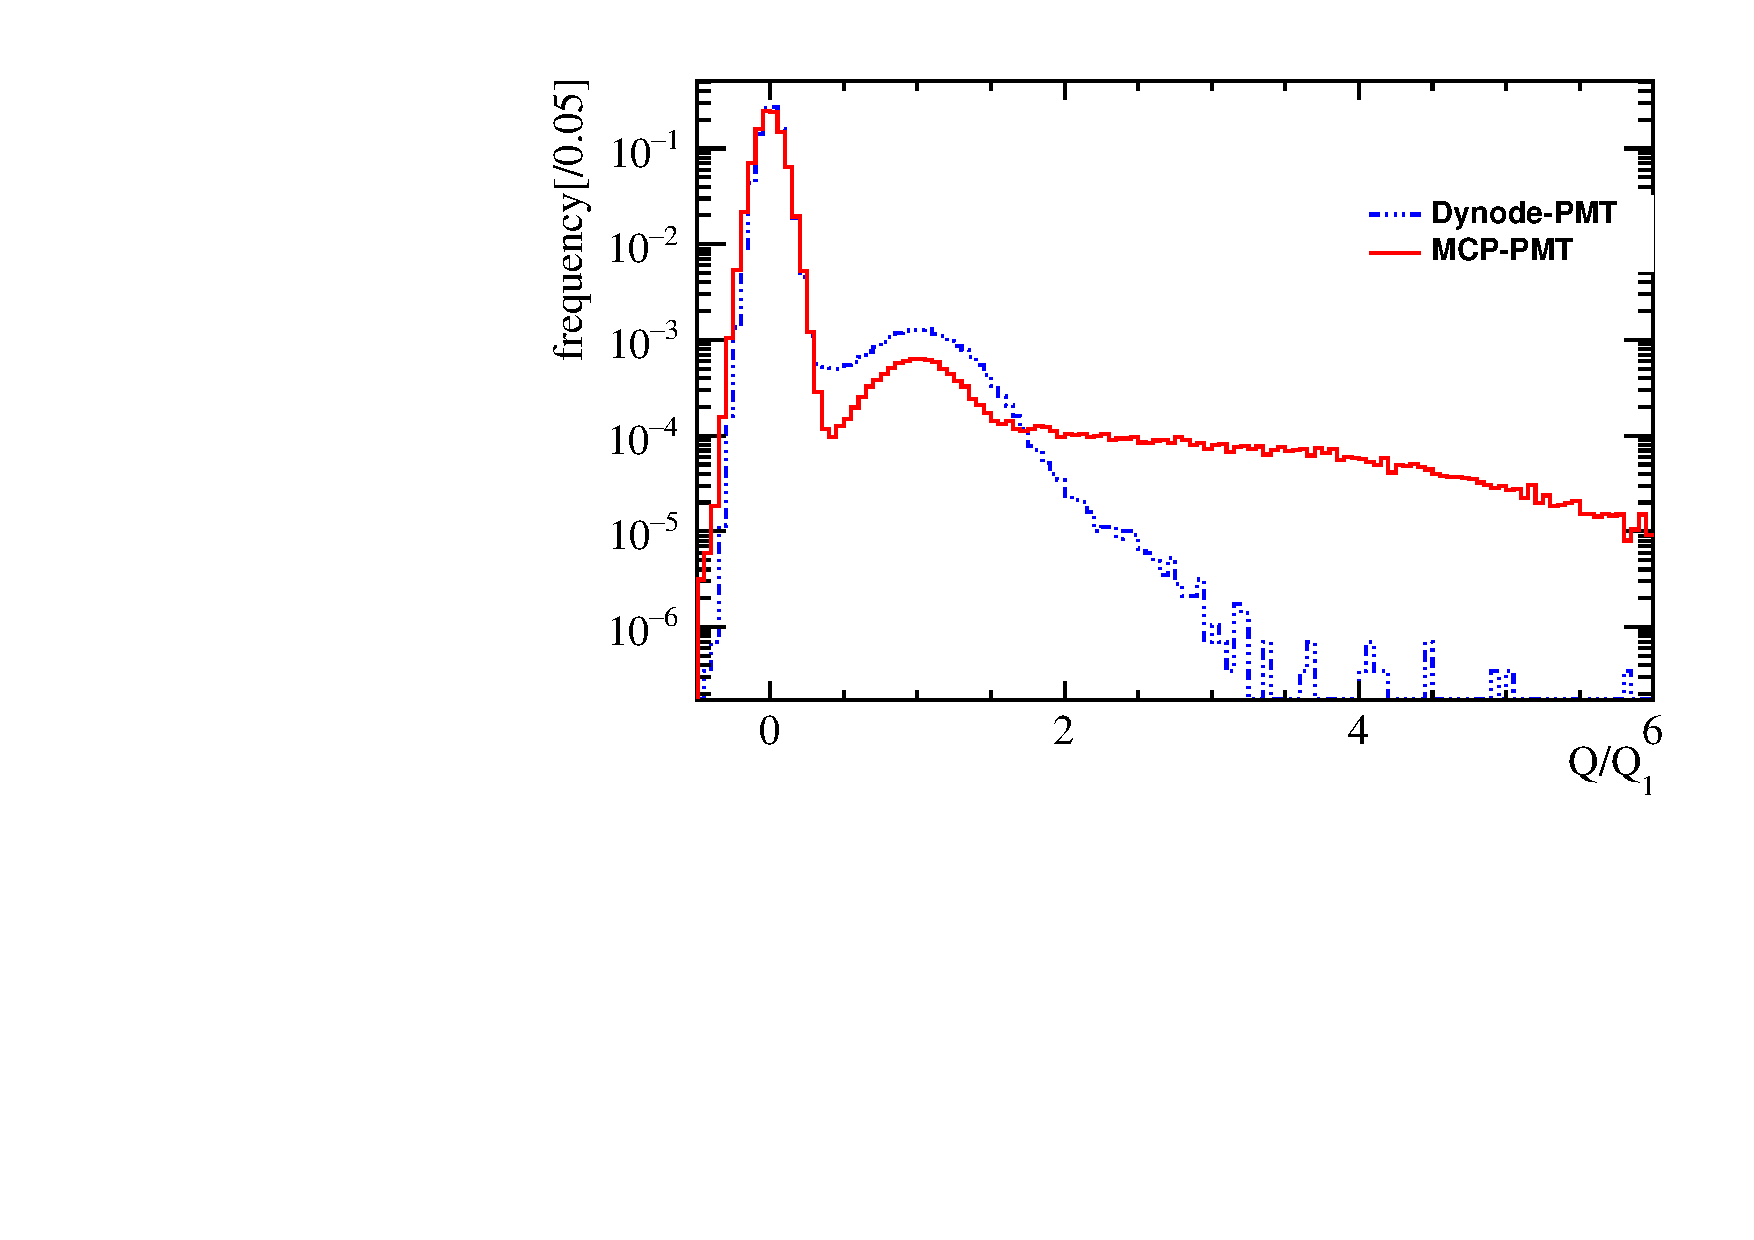
\includegraphics[width=0.7\linewidth]{spe.pdf_total.pdf}
    \caption{MCP-PMT 与 dynode PMT 单光电子电荷谱对比\cite{wengSingleElectronCharge2024}}
\end{figure}

其中 2. 与 3. 为该 MCP-PMT 的突出优点,并在测试\cite{zhangPerformanceEvaluation8inch2023} 中得到了验证。
同时,相较于传统 PMT 可以使用高斯分布描述的对称型单光电子响应电荷谱概率密度分布,4. 呈现的非对称长尾结构为使用该 PMT 带来了困难:
\begin{itemize}
    \item 分压实验研究\cite{yangMCPPerformanceImprovement2017} 中发现 MCP 对低能电子的增益远小于高能电子,揭示了单光电子电荷谱不能够认为只有单一的增益模式;
    \item 只截取主峰部分使用高斯分布拟合,则不能够充分利用长尾部分的信息,对提高统计量与能量分辨率没有帮助,
    且在没有充分物理认知的前提下直接使用主峰均值定义增益不具有坚实的理论依据;
    \item 在光强较强时,电荷谱将有多个峰结构,大电荷道址区域由电荷长尾与整数倍主峰共同贡献,直接拟合峰结构使得光电子数量估计有偏,进而引入能量偏差。
\end{itemize}

JUNO 采购了 15000 支 MCP-PMT 与 5000 支 dynode PMT,其中 20 寸 PMT 的光阴极覆盖率为 75.2\%,
在先行探测器 OSIRIS 上安装的 76 个大 PMT 也均为 20 寸 MCP-PMT,
因此 20 寸 MCP-PMT 的电荷增益刻度对提高探测器的能量分辨率具有重大的意义。
相较于其他应用 dynode PMT 的中微子探测器,JUNO 等探测器需要对新 PMT 展开仔细地刻度等研究,
增进对该类型 PMT 的理解与经验,尤其需要利用适合的电荷模型完成刻度,为 PMT 的信号读出提供坚实的物理基础,
进而达到提升能量分辨率的目标。
